% Copyright (c) 2024, Francisco Fernandez
% License: CC BY-SA 4.0
%   https://github.com/fernandezfran/thesis/blob/main/LICENSE
\subsection{Espectroscopia Mössbauer: División de picos}

Una perspectiva diferente en el estudio de la estructura atómica local puede 
obtenerse con la técnica espectroscópica de Mössbauer (MB), que consiste en medir 
la emisión o la absorción de rayos gamma asociada a las transiciones de niveles
de energía en el núcleo \cite{long2013}. Estos niveles de energía están 
influenciados por el entorno local, que puede cambiar o dividir estos niveles.
En la Figura \ref{fig:esquema-mossbauer} se presenta un esquema donde puede observarse un núcleo emisor de rayos $\gamma$ (en rojo) y un núcleo receptor (en verde), que corresponde a la muestra sobre la que se mide con un detector (en gris) si hay absorción o no de dichos rayos. En el gráfico de la derecha se muestran dos espectros típicos de Mössbauer. En el eje de las abscisas se tiene la velocidad, en mm/s, a la cual se hace oscilar el núcleo emisor de rayos $\gamma$, y en el eje de las ordenadas se tienen los dosespectros de absorción: ($\delta$) corresponde al desplazamiento isómerico en el cual el centro de la absorción está desplazado del cero y se debe a diferencias en el entorno de los electrones $s$ entre el núcleo emisor y el receptor; ($\Delta$) corresponde a la división cuadrupolar debida a las división de los niveles de energía nucleares cuando hay una distribución de carga no esférica y un número cuántico de momento angular $l$ mayor que 1/2.
\begin{figure}[h!]
    \centering
    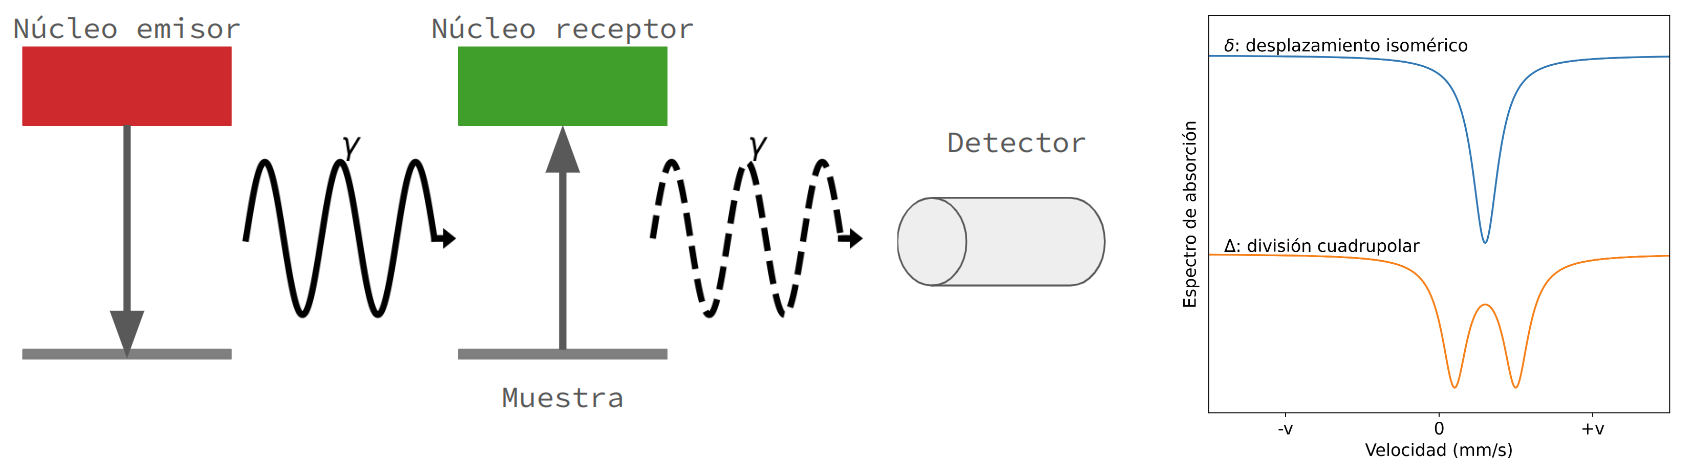
\includegraphics[width=\textwidth]{Silicio/prediccion/resultados/mossbauer/esquema_mossbauer.png}
    \caption{Esquema de la técnica de medición de espectroscopia Mössbauer que mide la emisión o absorción de rayos $\gamma$ asociada a las transiciones de niveles de energía en el núcleo.}
    \label{fig:esquema-mossbauer}
\end{figure}

Esta técnica fue utilizada por Li \textit{et al.} \cite{li2009} para medir los espectros de 
Mössbauer de rayos gamma de $^{119}$Sn en estructuras amorfas de 
Li$_x$Si$_{1-y}$Sn$_y$ para $0 < x < 3.5$ y valores pequeños de $y$. Se utilizó Sn debido a que el Si no es sensible a esta técnica de medición, mientras que el Sn sí lo es.
Dadas las concentraciones bajas de estaño, los autores suponen que los átomos de Sn
ocupan los mismos sitios que los de átomos de Si en este material, haciendo que 
las conclusiones inferidas para el Sn sean equivalentes para el Si 
\cite{hatchard2005}. La señal de MB en este sistema consiste de dos picos que se superponen casi 
completamente en los casos extremos de concentraciones bajas o altas de Li, 
pero están claramente separados para casos intermedios. Se espera que la distancia de separación
$\Delta$ sea sensible al entorno local de los átomos de Sn. $\Delta$
alcanza un valor máximo alrededor de $1.2$ mm/s para $x \sim 1$ y decrece para 
valores mayores o menores de $x$ (ver los triángulos en la Figura \ref{fig:mossbauer}).
\begin{figure}[h!]
    \centering
    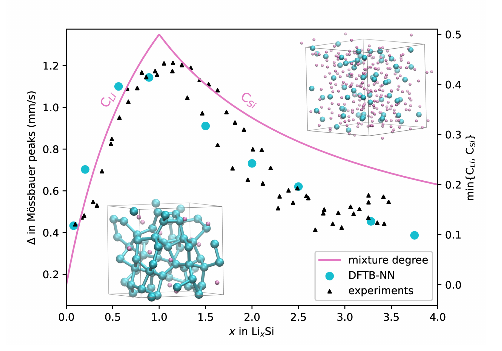
\includegraphics[width=.7\textwidth]{Silicio/prediccion/resultados/mossbauer/mossbauer.png}
    \caption{Separación entre los dos picos en los espectros de efecto 
    Mössbauer. Los triángulos que apuntan hacia arriba corresponden a dos 
    medidas de Li \text{et al.} \cite{li2009} (eje de la izquierda), la línea naranja discontinua es la 
    predicción de la ecuación \ref{eq:mossbauer}, utilizando concentraciones 
    globales de Li y Si. Los círculos azules son las predicciones dadas 
    por la ecuación \ref{eq:mossbauer}, con $C_{\text{Li}}$, $C_{\text{Si}}$ 
    calculados a partir de la concentración de los vecinos más cercanos (eje de 
    la derecha). Las barras de error son menores que el tamaño de los puntos.}
    \label{fig:mossbauer}
\end{figure}
Los autores sugieren que el valor máximo de $\Delta$ se obtiene cuando los átomos 
de Sn (y por analogía los de Si) están rodeados por una mezcla equimolar de Si y 
Li, y luego decrece cuando alguno de los dos tipos de átomos predomina. Con el fin 
de formular en términos cuantitativos esta idea, se define la concentración de 
átomos de Li ($C_{\text{Li}}$) y la concentración de átomos de Si 
($C_{\text{Si}}$) en términos del número de átomos de Li en la formula Li$_x$Si:
\begin{equation}\label{eq:clicsi}
    C_{\text{Li}} = \frac{x}{1+x} \hspace{2cm}y \hspace{2cm}  C_{\text{Si}} = 1 - C_{\text{Li}}.
\end{equation}
Ahora, como se observa en los datos experimentales de la Figura \ref{fig:mossbauer}
que $\Delta$ tiende a un valor constante para valores pequeños y grandes de $x$, 
se propone el siguiente \textit{ansatz} para $\Delta$:
\begin{equation}\label{eq:mossbauer}
    \Delta = a\min\left\lbrace C_{\text{Li}},C_{\text{Si}}\right\rbrace + b.
\end{equation}
Regulando los valores de $a$ y $b$ es posible ver (curva naranja discontinua en 
la Figura \ref{fig:mossbauer}) que esta dependencia simple produce la tendencia 
cualitativa del experimento. Sin embargo, la definición dada en la ecuación 
\ref{eq:clicsi} depende de la concentración promedio de Li en la aleación, mientras que 
MB percibe el entorno local. Se puede buscar una mejor concordancia si se calculan 
estos valores de concentraciones de Li y Si considerando los vecinos más cercanos
de cada átomo de Si para cada estructura amorfa obtenida en las simulaciones de
dinámica molecular. Si se reemplazan estos valores locales de $C_{\text{Li}}$ y 
$C_{\text{Si}}$ en la ecuación \ref{eq:mossbauer} se obtienen los puntos azules
de la Figura \ref{fig:mossbauer}, que muestran una mejora en la concordancia 
con los experimentos.
